\documentclass[
	classe=$1^{ere}STI2D$
]{exercice}

\usepackage{listings}
\usepackage{setspace}

\title{Exercices : probabilités}

\begin{document}

\maketitle

\begin{exercice}
	On lance deux dés : les premier est tétraédrique, et ses faces portent les numéros $1$, $1$, $2$ et $3$. Le deuxième est cubique, et ses faces portent les numéros $1$, $1$, $1$, $2$, $3$, $3$.

	On note $X$ la variable aléatoire égale à la somme des faces des deux dés.

	\begin{enumerate}
		\item Quelles sont les valeurs possibles de $X$ ?
		\item Représenter la situation par un arbre de probabilités.
		\item Déterminer la loi de probabilités de $X$, et la représenter dans un tableau.

		      \uline{Remarque} : on donnera les résultats sous forme fractionnaire.
		\item On veut écrire un algorithme qui simule l'expérience aléatoire, et qui détermine la moyenne des résultats obtenus pour $n$ simulations.

		      Compléter l'algorithme ci-dessous :

		      {\setstretch{1.15}\begin{lstlisting}[frame=single]
Fonction dés(n)
    m ← 0
    Pour i allant de 1 à ____
        d1 ← nombre entier aléatoire entre 1 et 4
        Si d1 = 4, alors
            d1 ← 1
        d2 ← nombre entier aléatoire entre _________
        Si d2 = 5 ou d2 = 6, alors
            d2 ← 1
        Si d2 = ____, alors
            d2 ← ____
        m ← m + d1 + d2
    m ← m ÷ ____
    Renvoyer m
\end{lstlisting}}
	\end{enumerate}
\end{exercice}

\begin{exercice}
	Lors d'un concours, un candidat doit répondre à un QCM contenant $4$ questions avec $3$ réponses possible à chaque fois. On note $X$ la variable aléatoire égale au nombre de bonnes réponses données par un candidat qui répond au hasard.
	\begin{enumerate}
		\item Donner la loi de probabilités de $X$ (les résultats seront donnés sous forme fractionnaire).
		\item Déterminer l'espérance de $X$, et écrire une phrase donnant l'interprétation de ce résultat dans le contexte de l'exercice.
		\item Le candidat gagne $1$ point par bonne réponse, mais perd $1$ point par mauvaise réponse. Les scores négatifs sont ramenés à $0$.

		      On note $Y$ la variable aléatoire égale au score obtenu.

		      Calculer $E(Y)$, et écrire une phrase donnant l'interprétation de ce résultat dans le contexte de l'exercice.
	\end{enumerate}
\end{exercice}

\begin{exercice}\

	\begin{minipage}{0.7\linewidth}
		On propose le jeu suivant : on tire une boule dans le sac. Si elle n'est pas marquée, on ne gagne rien. Si elle est marquée d'un trait, on gagne $5$€. Si elle est marquée d'une croix on gagne $10$€. On remet ensuite la boule dans le sac, et on en tire une autre avec les mêmes règles.

		Une partie coûte $8$€.
	\end{minipage}
	\begin{minipage}{0.25\linewidth}
		\begin{center}
			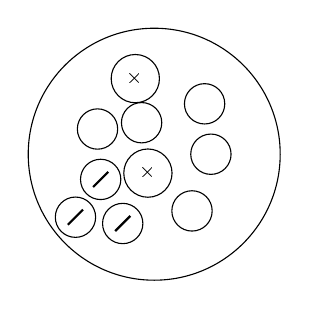
\begin{tikzpicture}[scale=0.8]
				\draw (0,0) circle (2);
				\foreach \x/\y in {-0.2/0.5,-0.9/0.4,0.9/0,0.6/-0.9,0.8/0.8} {
						\draw (\x,\y) circle (0.32);
					}
				\foreach \x/\y in {-0.1/-0.3,-0.3/1.2} {
						\node[circle,draw=black] at (\x,\y) {{\scriptsize ×}};
					}
				\foreach \x/\y in {-0.85/-0.4,-1.25/-1,-0.5/-1.1} {
						\draw (\x,\y) circle (0.32);
						\draw[thick] (\x,\y) ++(-0.12,-0.12) -- ++(0.24,0.24);
					}
			\end{tikzpicture}
		\end{center}
	\end{minipage}

	\begin{enumerate}
		\item Lors d'un tirage, quelle est la probabilité d'obtenir une boule bleue ?
		\item Représenter la situation par un arbre de probabilités.
		\item On note $X$ la variable aléatoire égale au gain algébrique (c'est-à-dire le gain moins la mise).
		      \begin{enumerate}
			      \item Calculer $P(X = 20)$.
			      \item Donner la loi de probabilités de $X$ sous forme de tableau.
			      \item Quelle est la probabilité de gagner ?
		      \end{enumerate}
	\end{enumerate}
\end{exercice}

\end{document}